\documentclass[border=1cm]{standalone}
\usepackage{tikz}
\usetikzlibrary{math}
\begin{document}

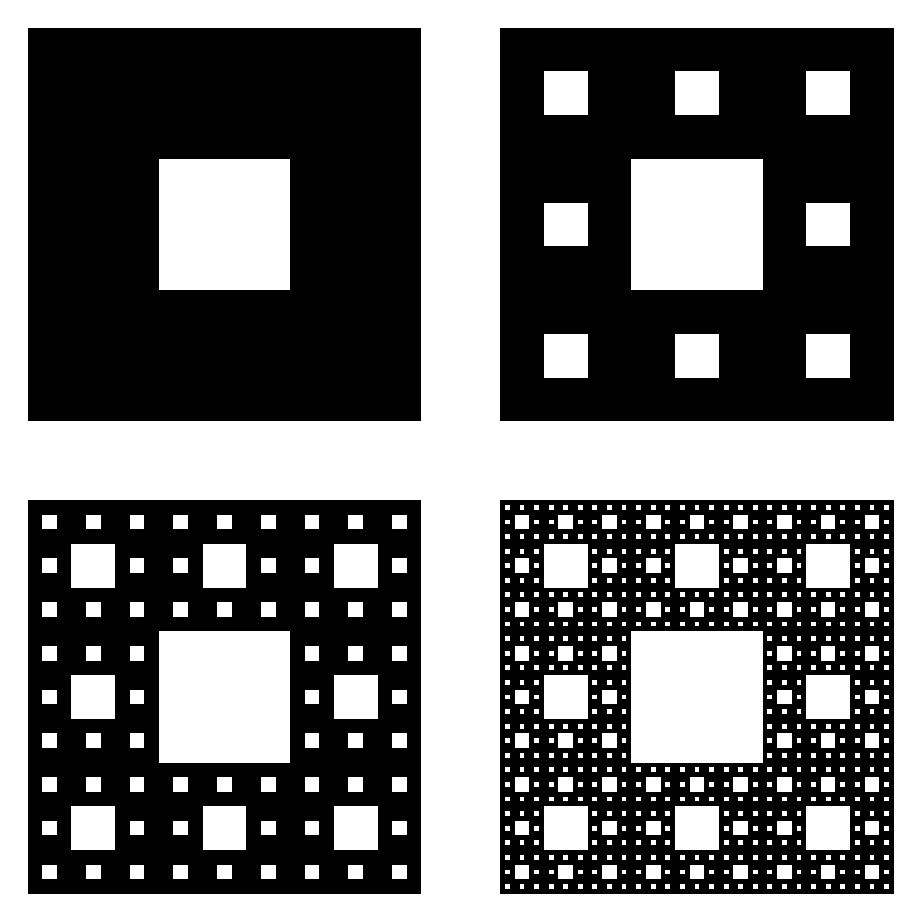
\begin{tikzpicture}
\tikzmath{
    function sierpinski_carpet(\x, \y, \s, \d) {
        if (\d == 0) then {
            { \fill[black] (\x, \y) rectangle (\x+\s, \y+\s); };
        } else {
            \ns = \s/3;
            for \ix in {0, 1, 2} {
                for \iy in {0, 1, 2} {
                    if (\ix == 1 && \iy == 1) then {
                        % Пропускаем центр (дырка)
                    } else {
                        sierpinski_carpet(\x + \ix*\ns, \y + \iy*\ns, \ns, \d-1);
                    };
                };
            };
        };
    };
}
% Вызов функции для 4 итераций
\tikzmath{ 
\S = 5;
for \d in {1,...,4}{
	% To situate all plots nicely under and next to each other, define the coords
	% of the lower left corners preemptively
	\x = (\S+1)*mod(\d-1,2);
	\y = int((\d-1)/2) * (\S+1);
	sierpinski_carpet(\x,-\y,\S,\d);
	};
}
\end{tikzpicture}

\end{document}